\section{Solenoid and Torus Magnets}


\subsection{Geometry}
The solenoid geometry is produced with the GEMC perl api. The solenoid is a single polycone volume, shown in \F{solenoid}
in a section view with the target and an 11 GeV electron beam.

\begin{figure}
	\centering
	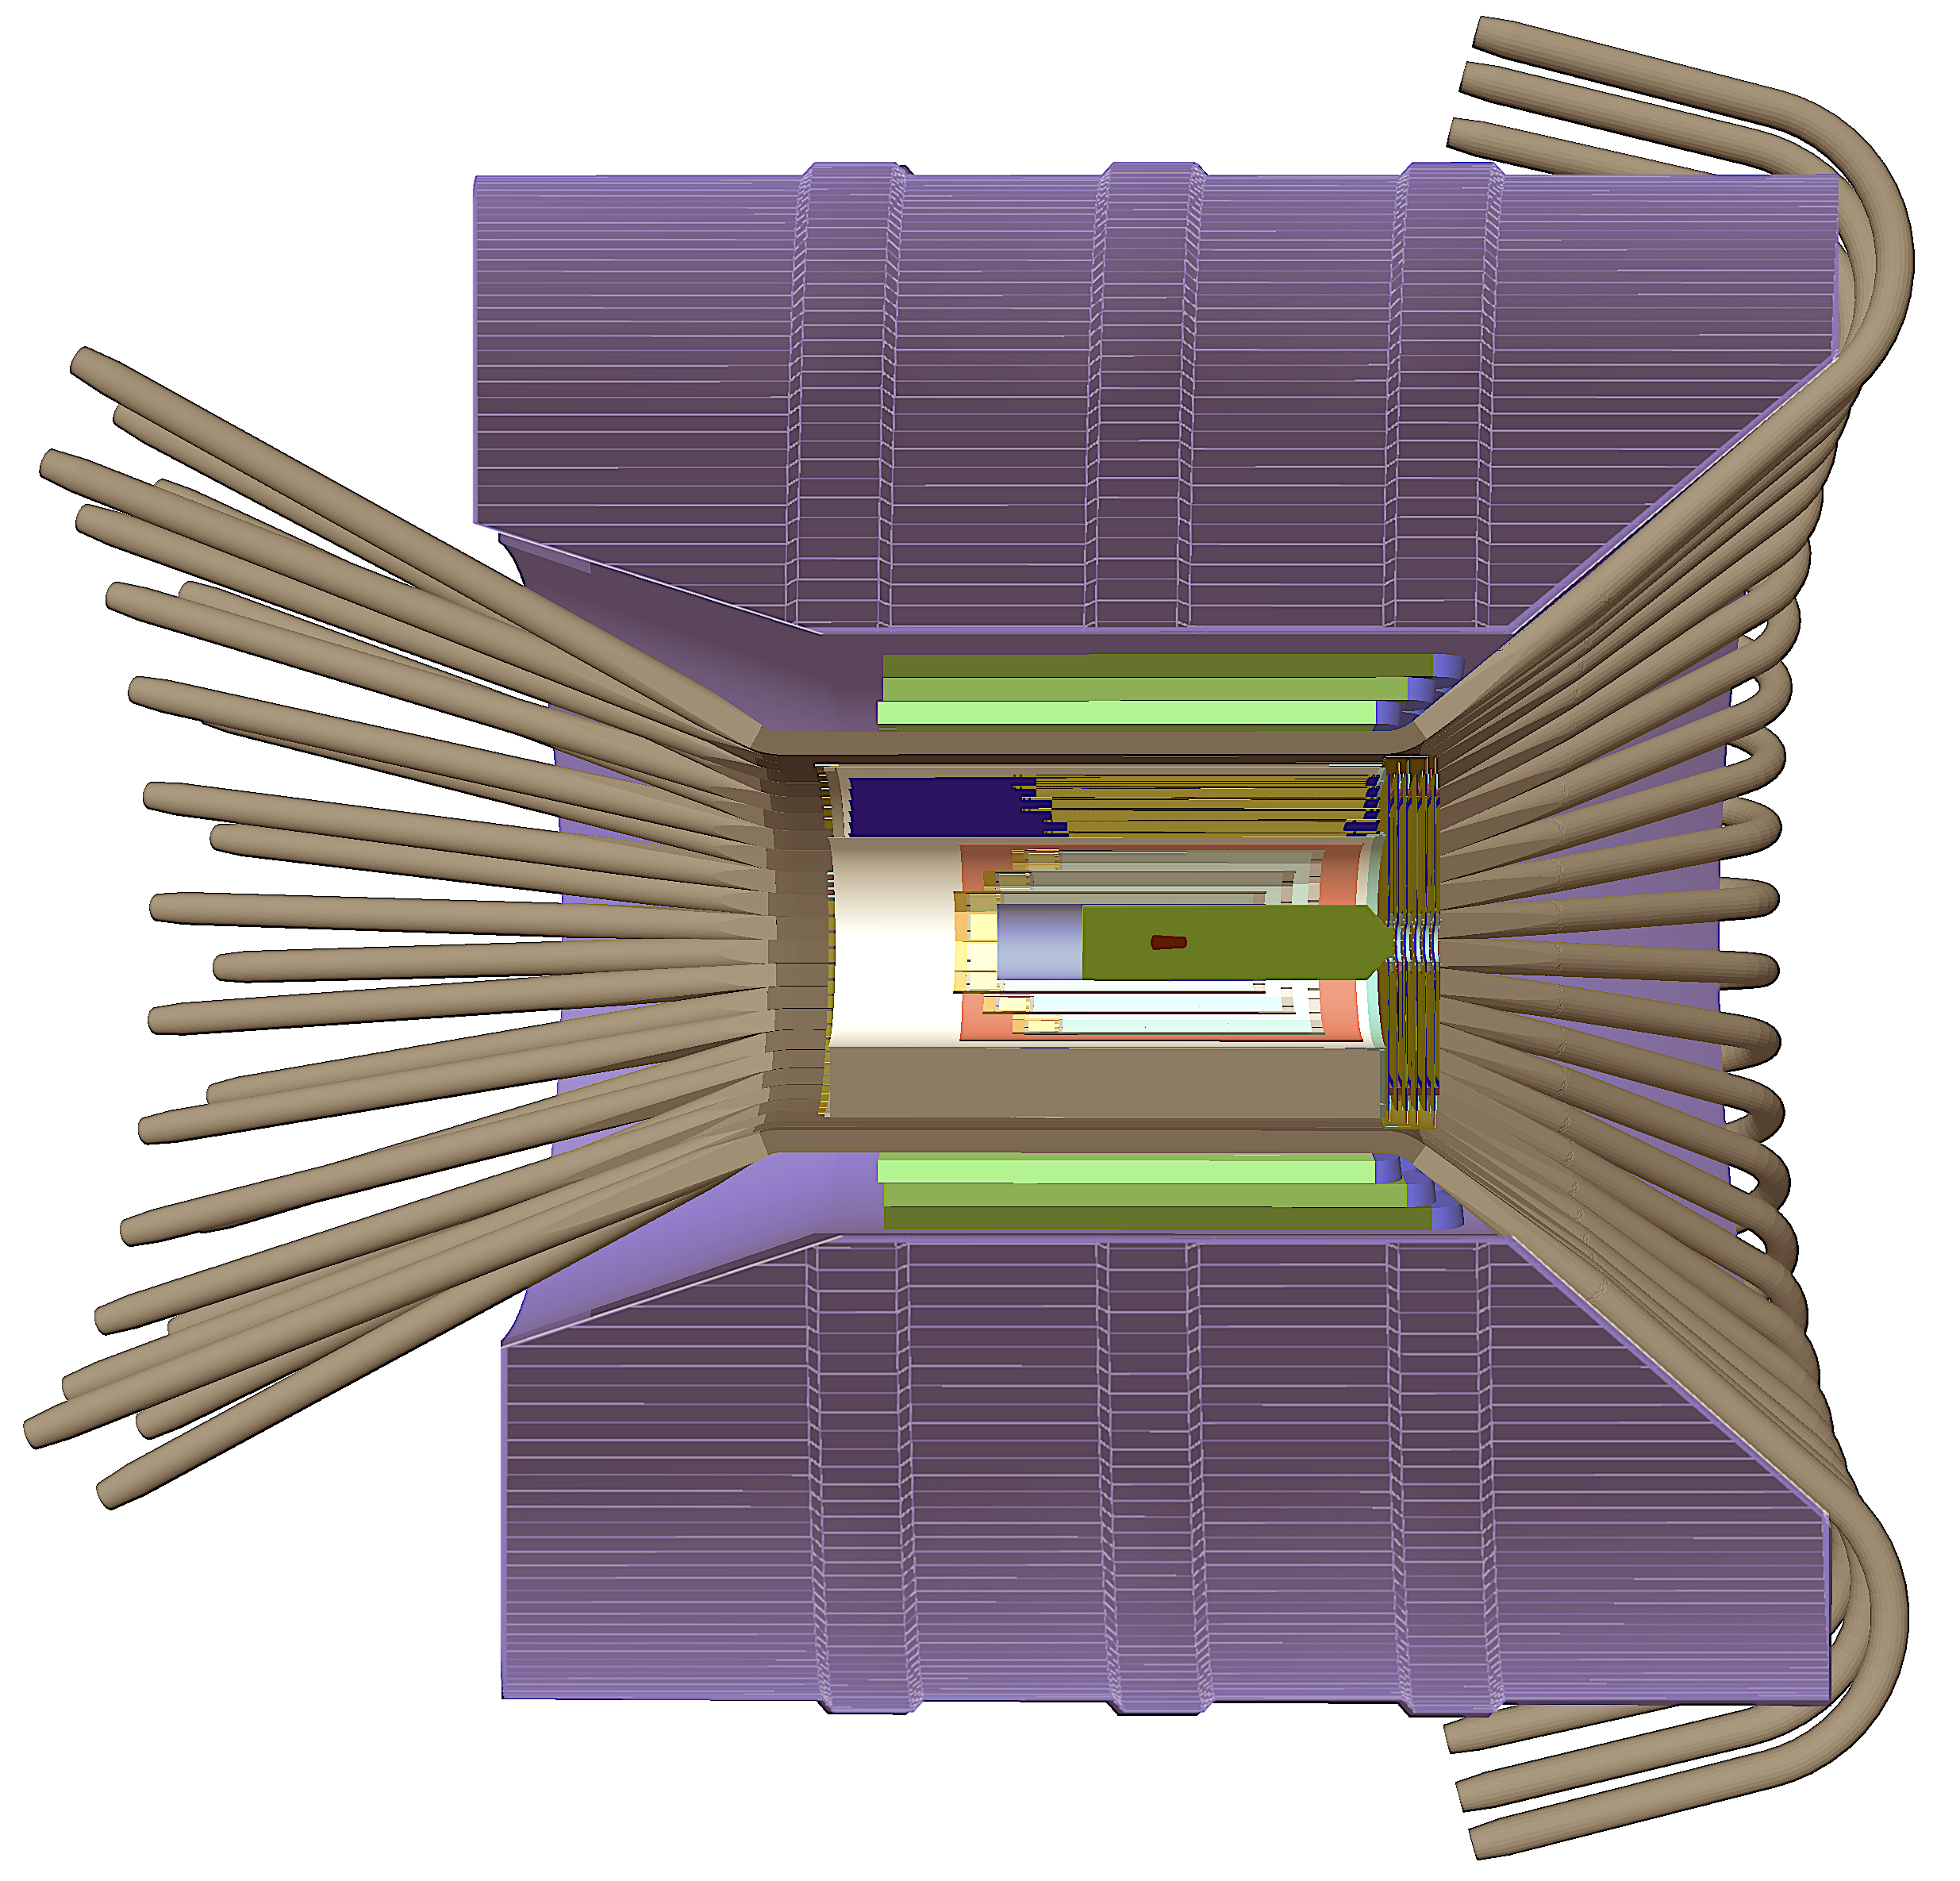
\includegraphics[width=0.98\columnwidth,keepaspectratio]{img/solenoid.png}
   \caption{An 11 GeV electron beam is impinging on a 5 cm liquid hydrogen target. At the full $10^{35} cm-2s-1$ luminosity, this correspond to
            124,000 electrons in a 250 ns window. Normally this would produce a storm of moeller electrons that would saturate any detector in the forward or central
				region. However the solenoid focus all of them along the beam line, providing the most effective shield to CLAS12.
            }
	\label{fig:solenoid}
\end{figure}

The torus geometry is imported from the engineering CAD model through 54 tessellated volumes. Among the volumes:

\begin{itemize}
	\item the bore heat shield and hub components
	\item the back and front plants
	\item the stainless steel coil frames
	\item the copper coils
	\item internal shielding around the hub
\end{itemize}

The torus hub is protected from the beampipe background with additional tungsten shielding.
The torus geometry is shown in \F{torus}.

\begin{figure}
	\centering
	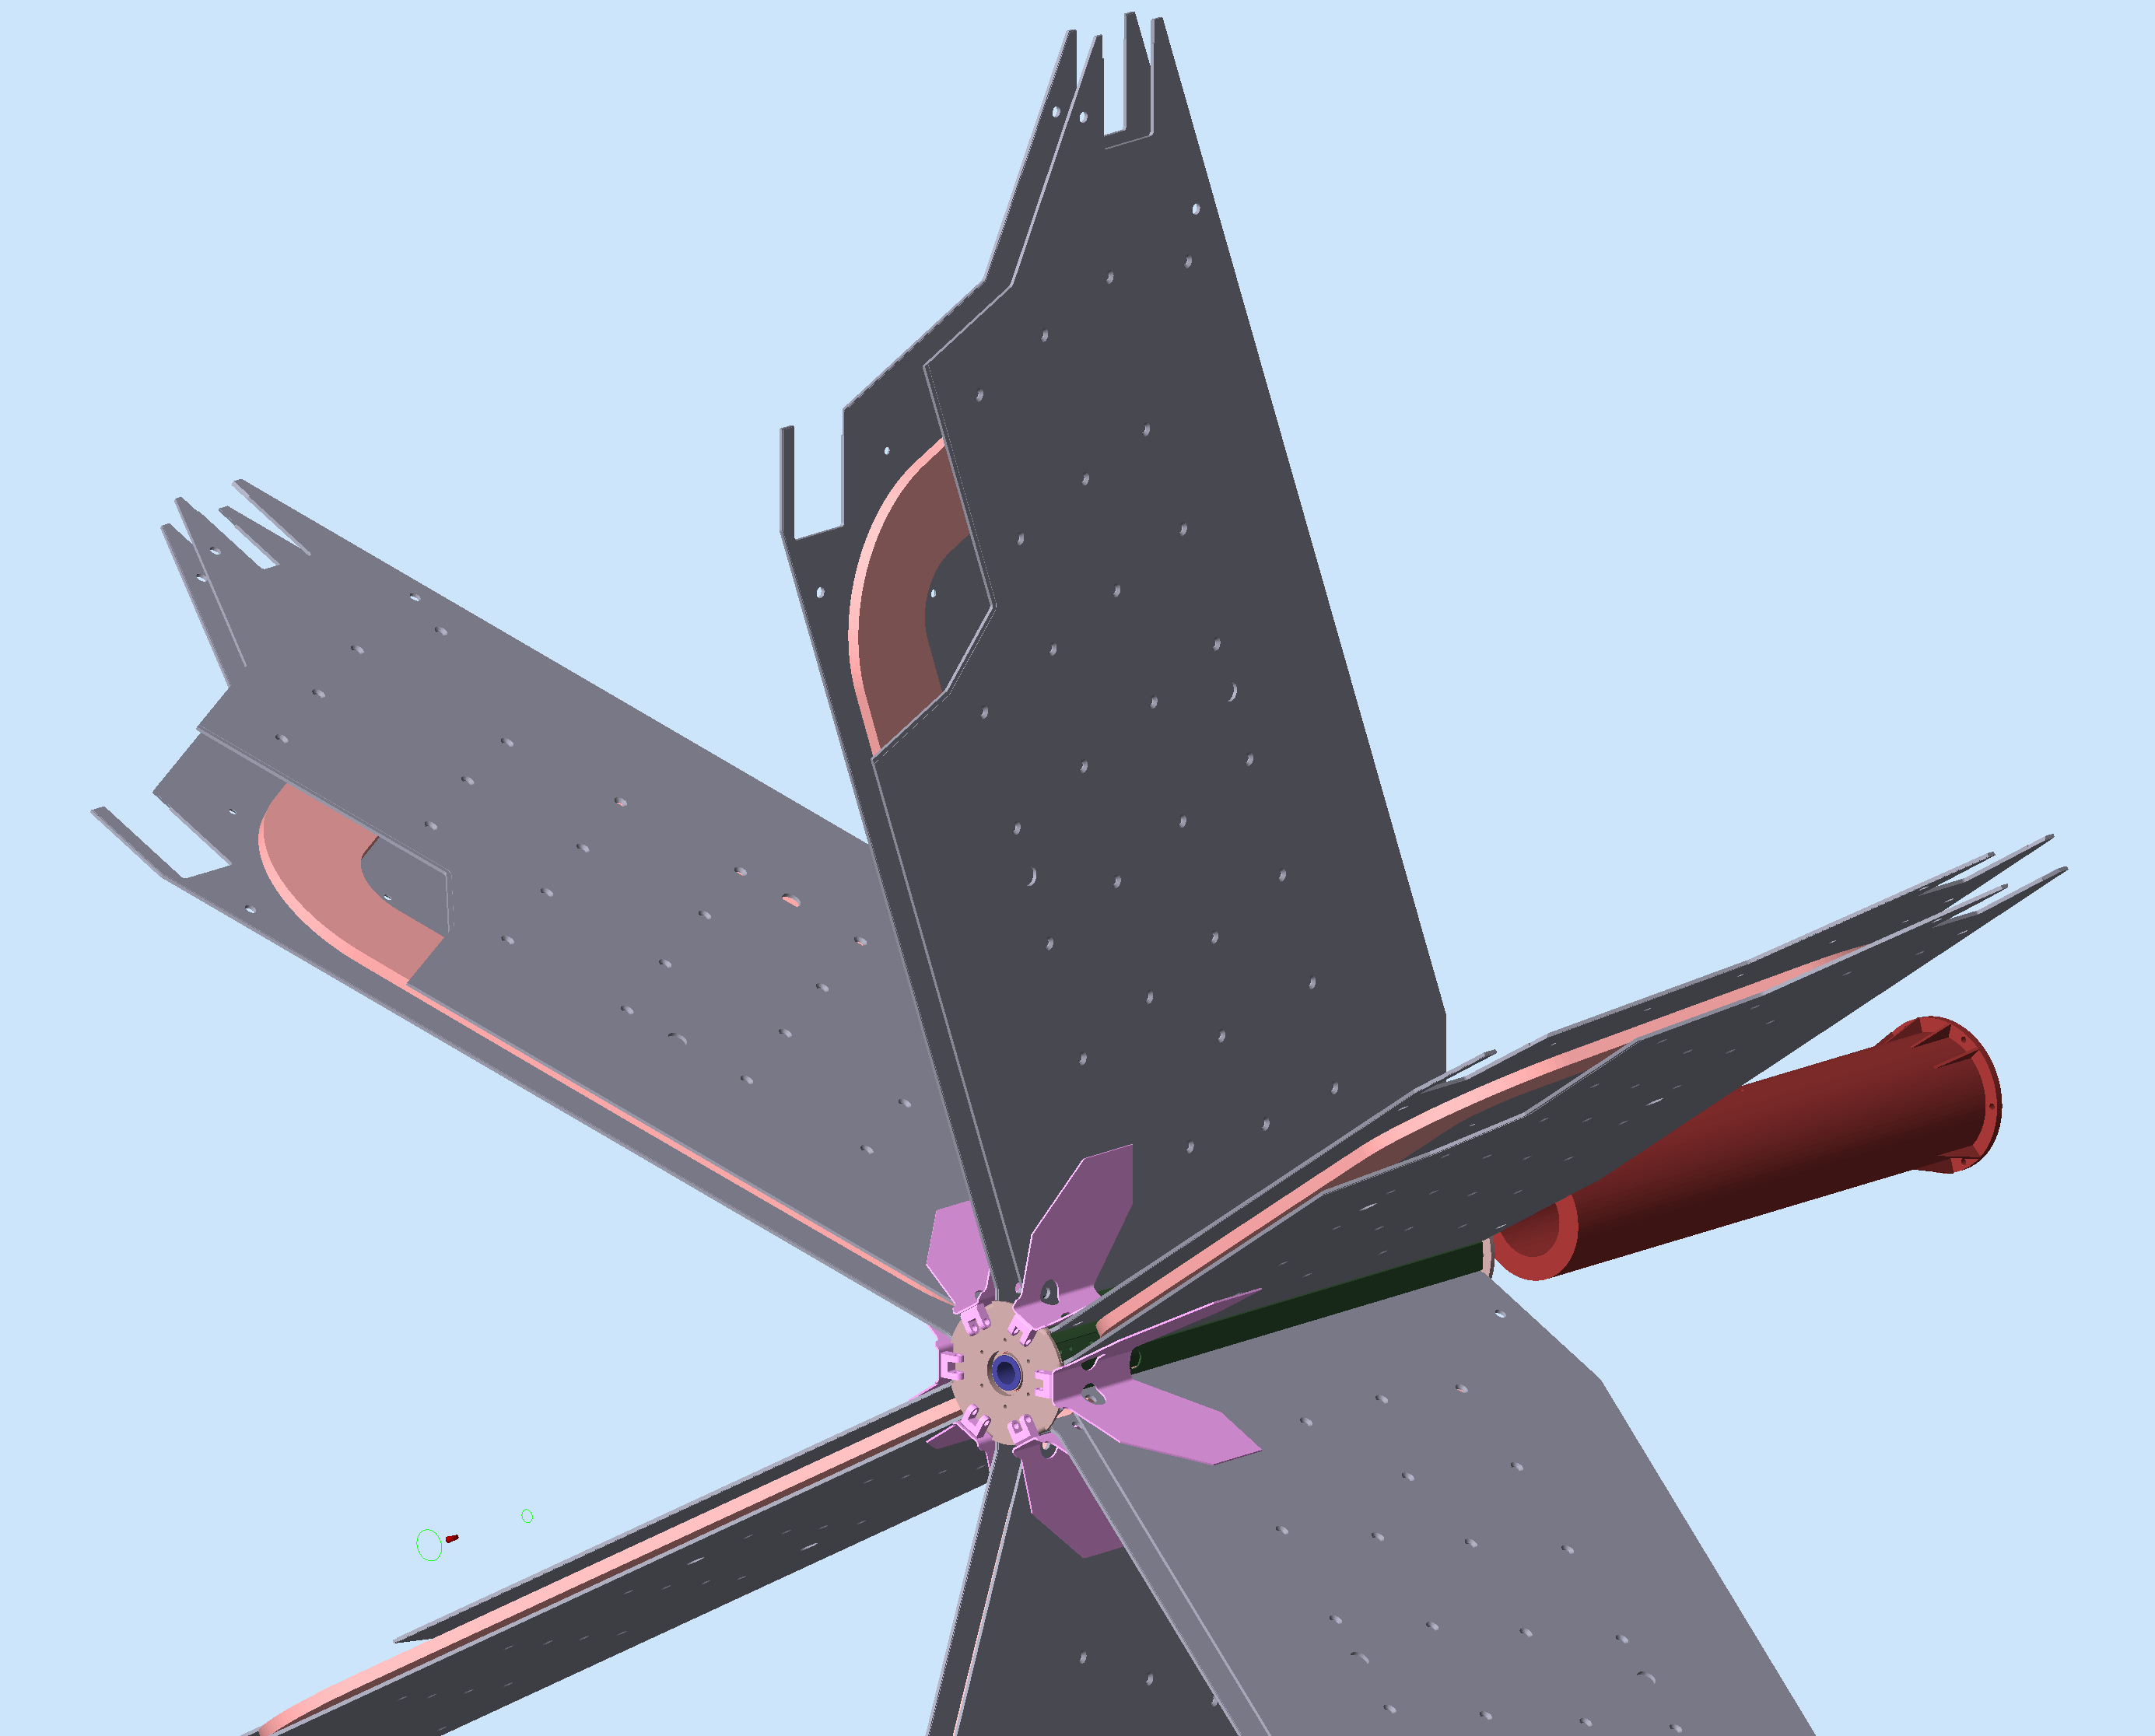
\includegraphics[width=0.95\columnwidth,keepaspectratio]{img/torusGeometry.png}
	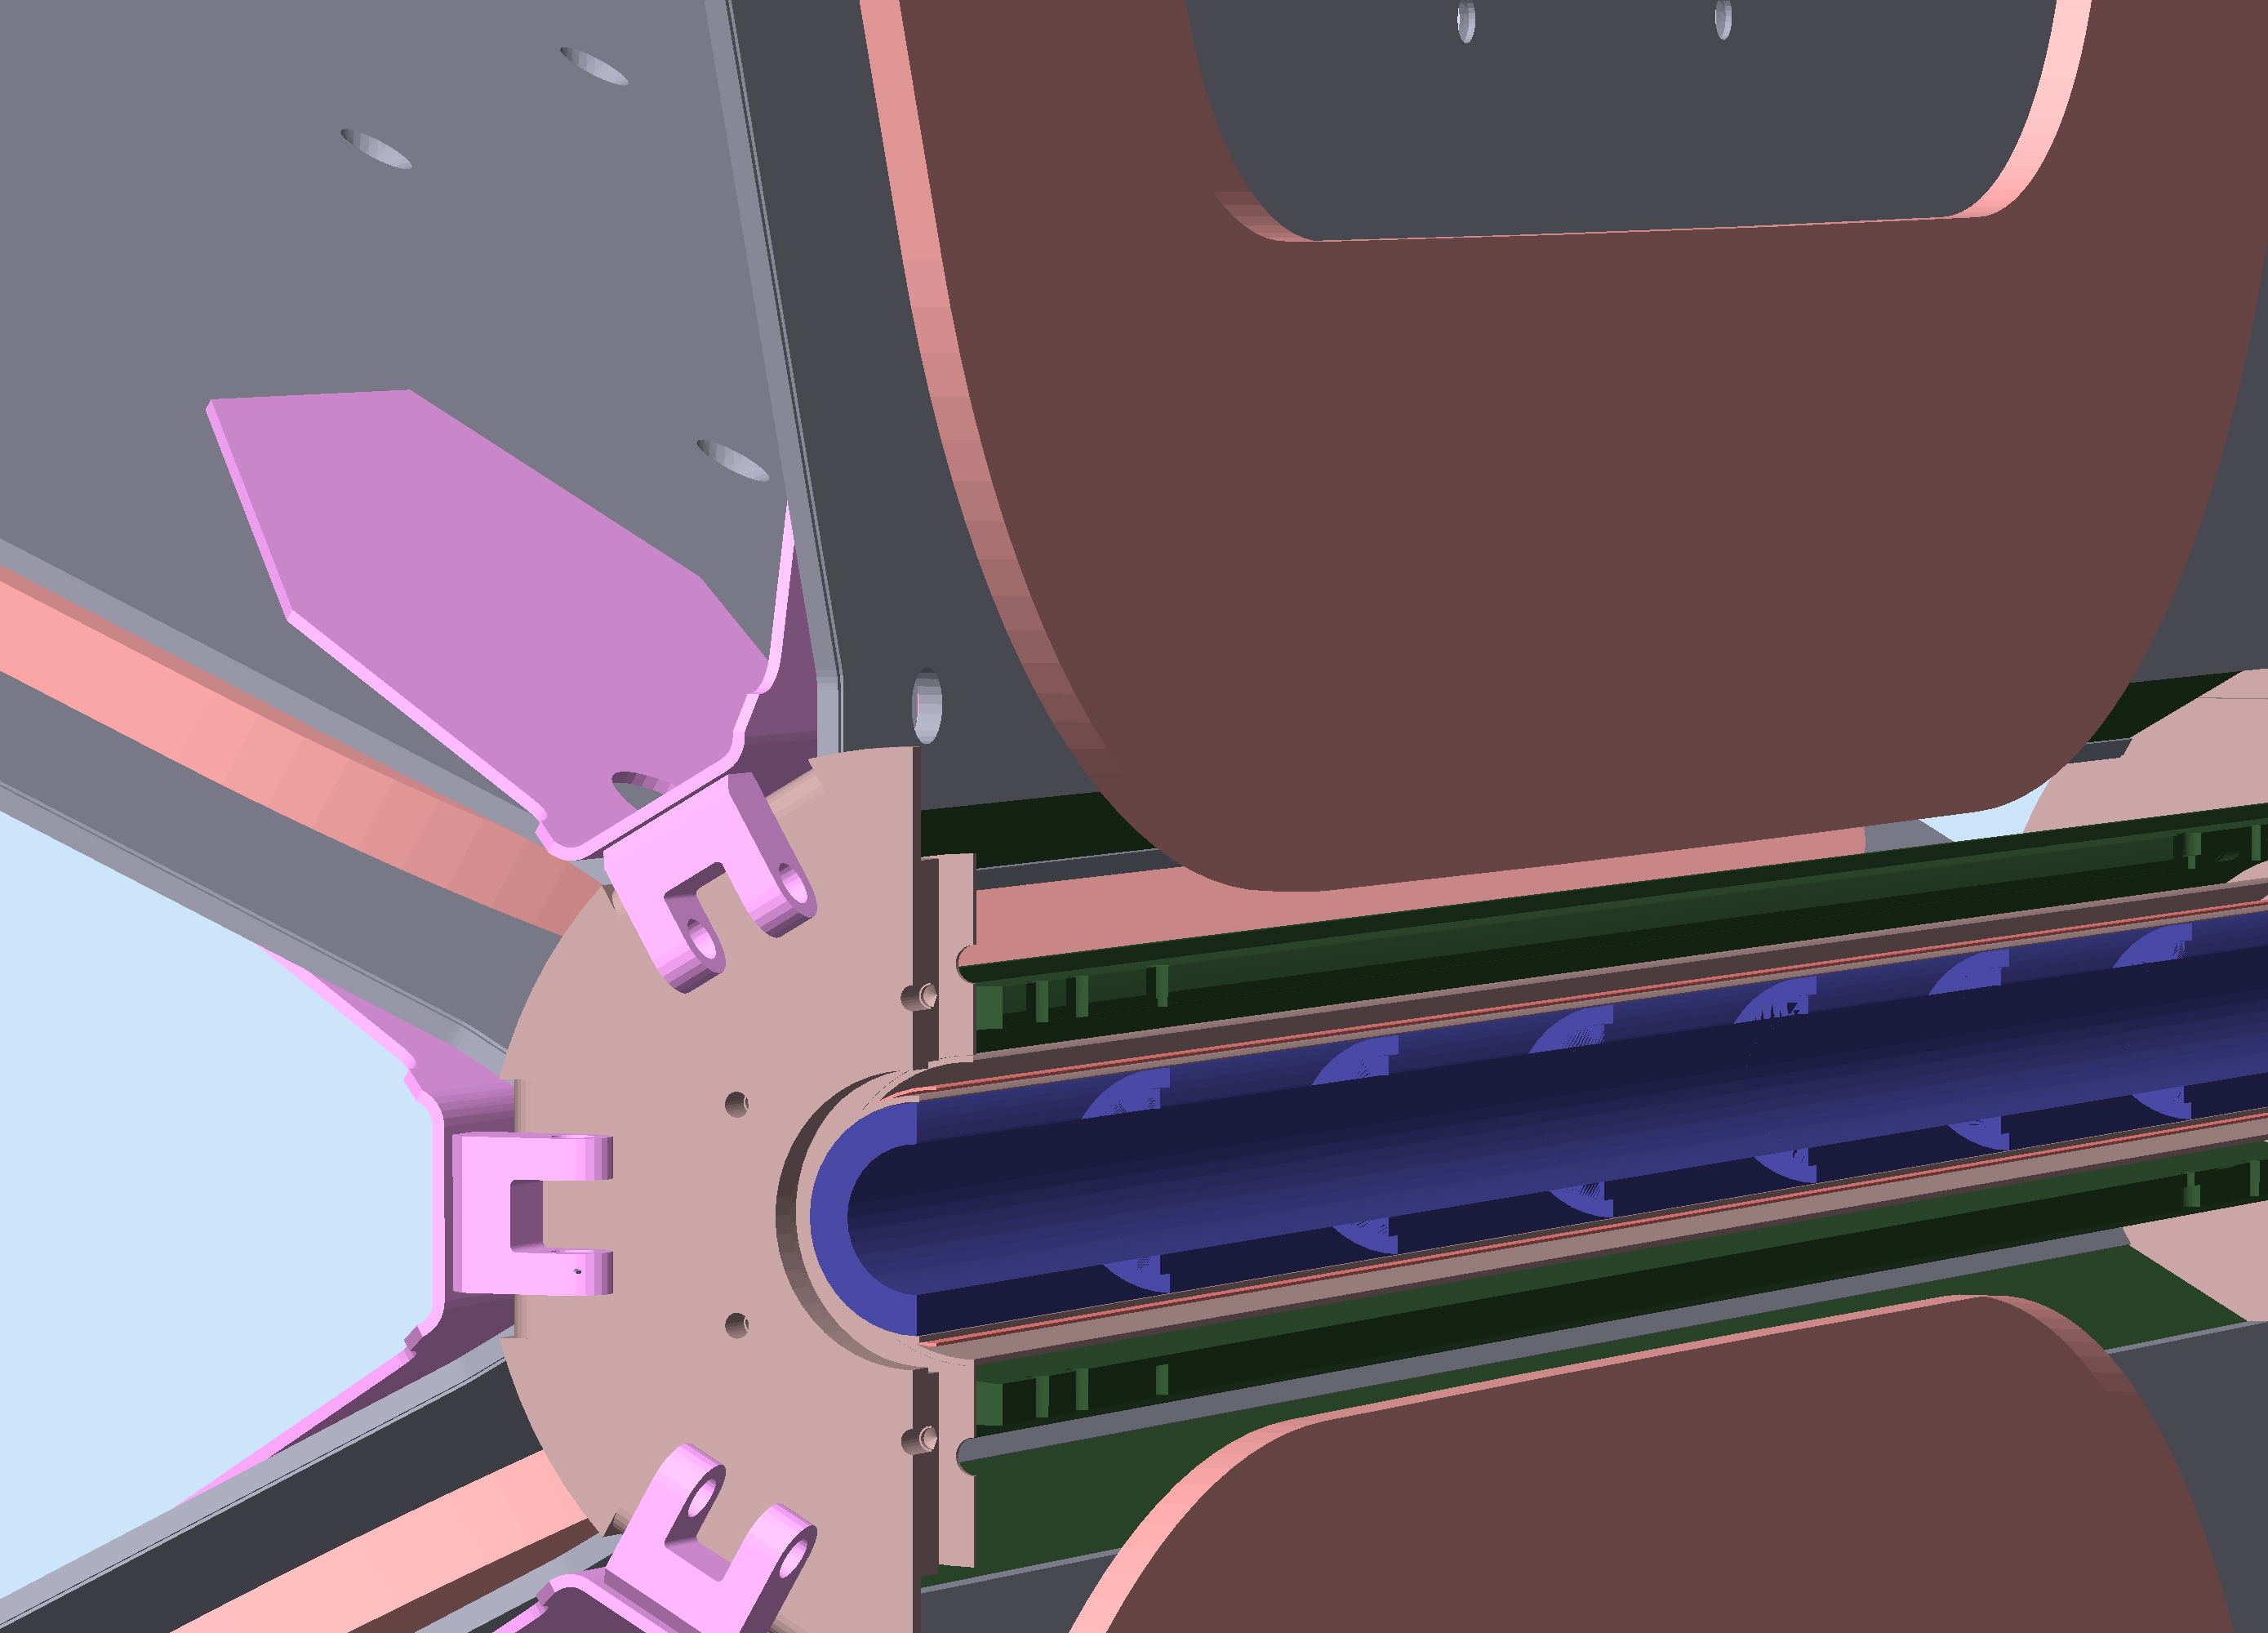
\includegraphics[width=0.95\columnwidth,keepaspectratio]{img/torusDetail.png}
	\caption{Top: the GEMC implementation of the torus hardware. The volumes are imported from the CAD engineering model.
            The stainless steel frame embeds the copper coils, immersed in the cold hub tube.
				Bottom: a section view of the torus in the vicinity of the beamline. The warm and cold hub are visible, along with the
				tungsten shielding (blue colors).}
	\label{fig:torus}
\end{figure}


\subsection{Magnetic Field Maps} \label{clas12FieldMaps}


The field maps are imported in the simulation using ascii files. Both fields can be scaled by an arbitrary number.
Both fields are defined in the Hall-B coordinate system and both can be shifted and tilted by additional delta amounts.

\subsubsection{Solenoid}
The solenoid field map has cylindrical symmetry around the z- axis, so the map is defined in the transverse / longitudinal plane
and then rotated when requested by the geant4 navigation. The integration method used in the simulation is the Range Kutta 4.

The solenoid field near the target points along the z direction and its uniformity is $\Delta B / B < 10^{-4}$.

The field map has 1200 points along the z-axis, from -3m to 3m. It has 600 points in the transverse coordinate, from 0 to 3m.
The field grid values are linearly interpolated to the (x,y,z) coordinate requested by geant4.

Table \ref{tab:solMap} shows the field map ascii data structure.


\begin{table}[h]
	\begin{center}
		\begin{tabular}{| c | c | c | c |}
			T (m)  & Z (m) &  $B_T $  & $ B_L $ \\
			\hline
          0.005  &  -0.025 & 0.000013  & 5.000880 \\
          0.005  &  -0.020 & 0.000044  & 5.000822 \\
          0.005  &  -0.015 & 0.000073  & 5.000704 \\
          0.005  &  -0.010 & 0.000101  & 5.000529 \\
          0.010  &  -0.025 & 0.000028  & 5.000928 \\
          0.010  &  -0.020 & 0.000089  & 5.000867 \\
          0.010  &  -0.015 & 0.000148  & 5.000747 \\
          0.010  &  -0.010 & 0.000203  & 5.000570 \\
		\end{tabular}
	\end{center}
	\caption{Solenoid ascii field map values around the target. The field values are in Tesla. $T=\sqrt(X^2+Z^2)$}\label{tab:solMap}
\end{table}

\subsubsection{Torus}
The torus field can be imported using a synmetric map or a full 3D map.
The symmetric map is defined in half the CLAS12 sector. It is symmetric around the sector midplane and copied in each sector
when requested by the geant4 navigation. The 3D map covers the entire cartesian space and accounts for field deviations due to coil
movements or imperfections.


The field map has 251 points along the z-axis, from 1m to 3m. It has 2501 points in the transverse coordinate, from 0 to 5m.
It has 16 azimuthal points from $0$ to $30^0$. The field grid values are linearly interpolated to the (x,y,z) coordinate requested by geant4.

The torus field in mid sector is perpendicular to the z-axis and is typically $2.5$ tesla.
Table \ref{tab:torMap} shows the field map ascii data structure.

\begin{table}[h]
	\begin{center}
		\begin{tabular}{| c | c | c | c | c | c | }
         $\phi$ (deg) & T (m)    & Z (m)    &  $B_x $  &    $B_y$    & $B_z$\\
			\hline
          0.0         &  190.0   &  338.0   &  0       &     4.51275 &  0 \\
          0.0         &  190.0   &  340.0   &  0       &     4.50136 &  0 \\
          0.0         &  190.0   &  342.0   &  0       &     4.48789 &  0 \\
          0.0         &  190.0   &  344.0   &  0       &     4.47235 &  0 \\
          0.0         &  190.0   &  346.0   &  0       &     4.45472 &  0 \\
          0.0         &  190.0   &  348.0   &  0       &     4.43502 &  0 \\
          0.0         &  190.0   &  350.0   &  0       &     4.41323 &  0 \\
          0.0         &  190.0   &  352.0   &  0       &     4.38935 &  0 \\
		\end{tabular}
	\end{center}
	\caption{Torus ascii field map values near mid-sector. The field values are in kGauss. $T=\sqrt(X^2+Z^2)$}\label{tab:torMap}
\end{table}


\subsubsection{Geometry Git Location}
The github location of the gemc perl api script for the solenoid and the torus CAD volumes is \url{https://github.com/gemc/detectors/tree/master/clas12/magnets}.

